O sistema de comunicação pode ser divido em 3 sub-sistemas principais:
\begin{itemize}
    \item Meio transmissor;
    \item Receptor;
    \item Transmissor;
\end{itemize}
No entanto, este trabalho foca exclusivamente no sistema transmissor, ilustrado pela figura \ref{fig:sistemadetrasmissao}, onde observa-se diversos elementos de que compõem o transmissor de sinal e dentre esses elementos tem-se que o amplificador de sinal é o componente de maior demanda energética, por se tratar do componente que converte a energia da fonte em energia irradiada pela antes de transmissão. Então para que o sistema de transmissão atue de maneira eficiênte é imprescindível que o trasmissor atue da maneira mais eficiênte o possivel. 

% // TODO Refazer figura
\begin{figure}[h!]
    \centering
    \captionsetup{justification=centering}
    \caption*{Fonte: autor}
    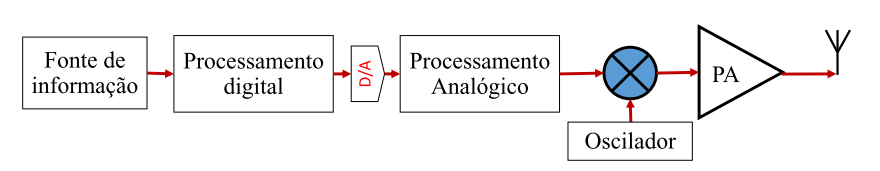
\includegraphics[width=0.5\textwidth]{sistematrasmissorpng.png}
    \caption{Sistema de transmissão simplificado}
    \label{fig:sistemadetrasmissao}
\end{figure}
